\section{Ứng dụng ma trận trong vật lý và cơ học}\label{sec_1}

Mục tiêu của phần này là sử dụng các tính chất của ma trận để tìm lại các kết quả đã trình bày trong tuần trước. Các kết quả trình bày dưới đây hoàn toàn có thể áp dụng được cho các hệ thống dao động phức tạp có nhiều bậc tự do hơn. Về mặt toán học hệ dao động 2 bậc tự do với các hệ dao động có 3,4,5 hoặc thậm chí 100 bậc tự do là tương tự.

\subsection{Dao động tự do}

Để làm quen với các khái niệm mới và ôn lại các phép toán ma trận, chúng ta sẽ sử dụng lại ví dụ về hệ dao động 2 bậc tự do đã trình bày trong tuần trước \cref{fig_2dofs}.

\begin{figure}[htbp]
    \centering
    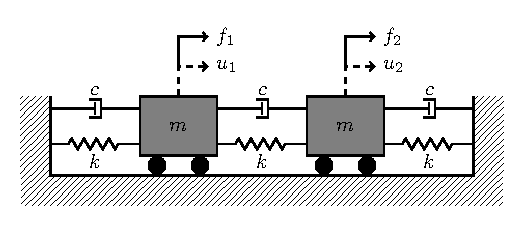
\includegraphics[width=1.\textwidth]{Tuan6/figure/mass_spring_damper_2dofs.pdf}
    \caption{2 dofs system}
    \label{fig_2dofs}
\end{figure}

Điều đầu tiên trong khảo sát một hệ thống dao động như trên hình đó là xác định các modes dao động riêng của hệ. Các modes dao động riêng của hệ là các modes mà ở đó tất cả các bậc tự do biến thiên theo thời gian với cùng tần số. Vì đây là một hệ thống tuyến tính nên nghiệm tổng quát (bất kỳ chuyển động nào của hai khối lượng) sẽ được thể hiện dưới dạng tổ hợp tuyến tính của các nghiệm liên quan đến từng chế độ. Để xác định các modes dao động riêng, ta bắt đầu với việc khảo sát hệ trong chế độ dao động tự do. Có nghĩa là $c=0$ và $f_1=f_2=0$. Ta có phương trình cân bằng cho hệ bên trên.

\begin{equation}\label{eq_PT2dofs}
    \begin{cases}
        m \ddot{u}_1 + 2ku_1 - ku_2 = 0 \\
        m \ddot{u}_2 + 2ku_2 - ku_1 = 0 \\
    \end{cases}
\end{equation}

Biểu diễn dưới dạng mà trận

\begin{equation}
    \label{eq_PTmatrix}
    \underbrace{\begin{bmatrix}
        m & 0\\ 0 & m
    \end{bmatrix}}_{\bf M}\underbrace{\begin{bmatrix}
        \ddot{u}_1 \\ \ddot{u}_2
    \end{bmatrix}}_{\ddot{\bf u}} +\underbrace{\begin{bmatrix}
        2k & -k \\ -k & 2k
    \end{bmatrix}}_{\bf K} \underbrace{\begin{bmatrix}
        u_1 \\ u_2
    \end{bmatrix}}_{\bf u} = \underbrace{\begin{bmatrix}
        0 \\ 0
    \end{bmatrix}}_{\bf O} 
\end{equation}

Các bậc tự do dao động với cùng sự phụ thuộc theo thời gian nên chúng ta có:

\begin{equation}
    {\bf u} = \begin{bmatrix}
        u_1 \\ u_2
    \end{bmatrix} = {\bf X}cos(\Omega t)
\end{equation}

Thay vào PT \cref{eq_PTmatrix} ta có:

\begin{equation}
    {\bf K}{\bf X} - \Omega^2{\bf M}{\bf X} = 0 \Leftrightarrow ({\bf K-\Omega^2{\bf M}}){\bf X} = 0
\end{equation}

Đây là một hệ phương trình tuyến tính với vế trái bằng 0. Để có nghiệm khác không, ma trận $\bf K-\Omega^2{\bf M}$ phải suy biến. Nghĩa là định thức của nó phải bằng 0:

\begin{equation}
    det({\bf K}-\Omega^2{\bf M}) = 0
\end{equation}

Đây là bài toán tìm trị riêng và vector riêng cua ma trận. Ta có thể giải bài toán này bằng cách sử dụng các hàm của Python như \textbf{numpy.linalg.eig} hoặc \textbf{scipy.linalg.eig}. Tuy nhiên vì đây là một ma trận $2\times 2$ nên ta có thể giải trực tiếp. Trị riêng (hay là tần số riêng) của ma trận này là nghiệm của phương trình bậc 2:

\begin{equation}
    \Omega^2 =  \Omega_1^2 = \frac{k}{m} \quad \hbox{va} \quad \Omega^2 = \Omega_2^2 = \frac{3k}{m}
\end{equation}

Vector riêng của hệ là

\begin{equation}
    {\bf X} = {\bf X}_1 = \begin{bmatrix}
        1 \\ 1
    \end{bmatrix} \quad \hbox{và} \quad {\bf X} = {\bf X}_2 = \begin{bmatrix}
        1 \\ -1
    \end{bmatrix}
\end{equation}

Nghiệm tổng quát của hệ là tổ hợp tuyến tính của hai modes này. Ta có thể viết lại nghiệm tổng quát của hệ như sau:

\begin{equation}
    {\bf u}=\underbrace{\left(A_1 \cos \left(\Omega_1 t\right)+B_1 \sin \left(\Omega_1 t\right)\right) {\bf X}_1}_{\hbox{Mode 1}}+\underbrace{\left(A_2 \cos \left(\Omega_2 t\right)+B_2 \sin \left(\Omega_2 t\right)\right) {\bf X}_2}_{\hbox{Mode 2}}
\end{equation}

Các hằng số $A_1, B_1, A_2, B_2$ được xác định từ các điều kiện ban đầu của hệ. Ví dụ nếu ta biết vận tốc và vị trí ban đầu của hai khối lượng thì ta có thể xác định được các hằng số này.

\subsection{Dao động cưỡng bức - Không có giảm chấn}

Xét trường hợp $f_1 = F_1\cos(\omega t)$ va $f_2 = F_2\cos(\omega t)$. Đặt ${\bf f} = \begin{bmatrix} F_1 \\ F_2\end{bmatrix}\cos(\omega t) = {\bf F}\cos(\omega t)$. Nghiệm của PT lúc này có dạng ${\bf u} = \begin{bmatrix} U_1 \\ U_2\end{bmatrix}\cos(\omega t) = {\bf U}\cos(\omega t)$. Thay vào PT \cref{eq_PTmatrix}, ta có:

\begin{equation}
    -\omega^2{\bf M}{\bf U} + {\bf K}{\bf U} = {\bf F} \Rightarrow {\bf U} = (-\omega^2{\bf M}+{\bf K})^{-1} {\bf F}
\end{equation}

Ta tìm được giá trị của $U_1$ va $U_2$

\begin{equation}
    U_1 = \frac{F_1(2k-m\omega^2)+F_2k}{(k-m\omega^2)(3k-m\omega^2)} \quad \hbox{và} \quad U_2 = \frac{F_1k+F_2(2k-m\omega^2)}{(k-m\omega^2)(3k-m\omega^2)}
\end{equation}

\subsection{Dao động cưỡng bức - có giảm chấn}

Trường hợp hệ số giảm chấn  $c \neq 0$, phương trình cân bằng được viết lại như sau:

\begin{equation}\label{eq_PT2dofs_c}
    \begin{cases}
        m \ddot{u}_1 + 2c\dot{u}_1 - c\dot{u}_2 + 2ku_1 - ku_2 = f1 \\
        m \ddot{u}_2 + 2c\dot{u}_2 - c\dot{u}_1 + 2ku_2 - ku_1 = f2 \\
    \end{cases}
\end{equation}

Dạng ma trận của phương trình này là:

\begin{equation}\label{eq_PT2dofs_c_matrix}
    \underbrace{\begin{bmatrix}
        m & 0\\ 0 & m
    \end{bmatrix}}_{\bf M}\underbrace{\begin{bmatrix}
        \ddot{u}_1 \\ \ddot{u}_2
    \end{bmatrix}}_{\ddot{\bf u}} + \underbrace{\begin{bmatrix}
        2c & -c \\ -c & 2c
    \end{bmatrix}}_{\bf C}\underbrace{\begin{bmatrix}
        \dot{u}_1 \\ \dot{u}_2
    \end{bmatrix}}_{\dot{\bf u}} +\underbrace{\begin{bmatrix}
        2k & -k \\ -k & 2k
    \end{bmatrix}}_{\bf K} \underbrace{\begin{bmatrix}
        u_1 \\ u_2
    \end{bmatrix}}_{\bf u} = \underbrace{\begin{bmatrix}
        f_1 \\ f_2
    \end{bmatrix}}_{\bf f} 
\end{equation}

Để giải phương trình này, chúng ta sẽ viết nó về dạng số phức. Vector ngoại lực ${\bf f}$ lúc này sẽ được biểu diễn ở dạng phức ${\bf f} = {\bf F}e^{j\omega t}$. Nghiệm của phương trình sẽ có dạng ${\bf u} = {\bf U}e^{j\omega t}$.

Thay vào phương trình \cref{eq_PT2dofs_c_matrix} ta có (\textcolor{red}{việc biến đổi để suy ra nghiệm dưới đây là một bài tập dành cho các bạn}):

\begin{equation}\label{eq_nghiemphuc}
    \begin{aligned}
        {U}_1 &=\frac{\left(2 F_1+F_2\right) k-F_1 m \omega^2+j c\left(2 F_1+F_2\right) \omega}{\left(j c \omega+k-m \omega^2\right)\left(3 j c \omega+3 k-m \omega^2\right)}\\
        {U}_2 &=\frac{\left(F_1+2 F_2\right) k-F_2 m \omega^2+j c\left(F_1+2 F_2\right) \omega}{\left(j c \omega+k-m \omega^2\right)\left(3 j c \omega+3 k-m \omega^2\right)}
    \end{aligned}
\end{equation}

Biên độ của $U_1$ và $U_2$:

\begin{equation}
    \begin{aligned}
         \left|U_1\right|&=\frac{\sqrt{\left(2 c F_1 \omega+c F_2 \omega\right)^2+\left(2 F_1 k+F_2 k-F_1 m \omega^2\right)^2}}{\sqrt{c^2 \omega^2+\left(k-m \omega^2\right)^2} \sqrt{9 c^2 \omega^2+\left(m \omega^2-3 k\right)^2}} \\
         \left|U_2\right|&=\frac{\sqrt{\left(c F_1 \omega+2 c F_2 \omega\right)^2+\left(F_1 k+2 F_2 k-F_2 m \omega^2\right)^2}}{\sqrt{c^2 \omega^2+\left(k-m \omega^2\right)^2} \sqrt{9 c^2 \omega^2+\left(m \omega^2-3 k\right)^2}}\\
    \end{aligned}
\end{equation}

\textbf{\textcolor{red}{Câu hỏi: chúng ta sẽ giải quyết bài toán như thế nào nếu ${\bf f}$ có dạng ${\bf f} = {\bf F}_1\cos(\omega_1t) + {\bf F}_2\sin(\omega_2t)$ ?}}

\subsection{Giải PT dao động tổng quát}

Phan nay se trinh bay cach giai phuong trinh dao dong tong quat khi co giam chan ($c \neq 0$) va vector ngoai luc la 1 ham bat ky. 

\begin{equation}\label{eq_PT_general}
    {\bf M}\ddot{\bf u} + {\bf C}\dot{\bf u} + {\bf K}{\bf u} = {\bf f}
\end{equation}

Luc nay viec tim nghiem cua phuong trinh la bat kha thi. Thay vao do chung ta se quan tam den gia tri cua nghiem tai 1 thoi diem nao do. De lam duoc viec nay chung ta se bat dau bang viec roi rac hoa thoi gian va su dung cac thuat toan vong lap de xap xi nghiem cua PT tai 1 thoi diem xac dinh.

Miền tích phân thời gian cũng sẽ được rời rạc hóa thành các bước thời gian $t_0, t_1, t_2, t_3, t_4, \dots, t_n$ với $\Delta t = (t_n-t_0)/n$.

Phuong phap Runge-Kutta va phuong phap Newmark se duoc trinh bay trong phan nay. Day la 2 trong so nhung phuong phap pho bien nhat de giai phuong trinh vi phan.

\subsubsection{Phương pháp Runge-Kutta}

Một trong những phương pháp số để tính toán phương trình dạng này là phương pháp Runge-Kutta. Phương pháp này là một phương pháp lặp để giải phương trình đạo hàm bậc nhất.

\begin{equation}
    \frac{d {\bf u}}{d t}={\bf f}(t,{\bf u}) ,\quad {\bf u}\left(t_0\right)={\bf u}_0
\end{equation}

PP Runge-Kutta xap xi nghiem tai buoc thoi gian $t_{n+1}$ dua tren gia tri tai buoc thoi gian truoc do $t_n$. Gia tri tai buoc thoi gian $t_{n+1}$ duoc tinh toan nhu sau:

\begin{equation}
    {\bf u}_{n+1} = {\bf u}_n + h \sum_{i=1}^s b_i {\bf k}_i
\end{equation}

\begin{equation}
\begin{aligned}
     {\bf k}_1 & = {\bf f}(t_n, {\bf u}_n), \\
     {\bf k}_2 & = {\bf f}(t_n+c_2h, {\bf u}_n+h(a_{21}{\bf k}_1)), \\
     {\bf k}_3 & = {\bf f}(t_n+c_3h, {\bf u}_n+h(a_{31}{\bf k}_1+a_{32}{\bf k}_2)), \\
         & \ \ \vdots \\
     {\bf k}_s & = {\bf f}(t_n+c_sh, {\bf u}_n+h(a_{s1}{\bf k}_1+a_{s2}{\bf k}_2+\cdots+a_{s,s-1}{\bf k}_{s-1})).
\end{aligned}
\end{equation}

Cac gia tri $a_{ij}, b_i, c_i$ duoc trinh bay theo ma tran Butcher. Ma tran Butcher duoc viet nhu sau:

\begin{equation}
\begin{array}{c|cccc}
0      &        &        &        &        \\
c_{2}  & a_{21} &        &        &        \\
c_{3}  & a_{31} & a_{32} &        &        \\
\vdots & \vdots & \vdots & \ddots &        \\
c_{s}  & a_{s1} & a_{s2} & \cdots & a_{s,s-1} \\
\hline
       & b_{1}  & b_{2}  & \cdots & b_{s}
\end{array}   
\end{equation}

Ma tran Bucher cho cac phuong phap Runge-Kutta bac 2, bac 4 (RK4) va Runge-Kutta 3/8 duoc trinh bay duoi day.

Runge-Kutta bậc 2
\begin{equation}
    \begin{array}{c|cccc}
    0 & & \\
    1/2 & 1/2 & \\
    \hline
    & 0 & 1
    \end{array}   
\end{equation}

Runge-Kutta bậc 4 (RK4)
\begin{equation}
    \begin{array}{c|cccc}
        0 & & & & \\
        1/2 & 1/2 & & & \\
        1/2 & 0 & 1/2 & & \\
        1 & 0 & 0 & 1 &\\
        \hline
        & 1/6 & 1/3 & 1/3 & 1/6
    \end{array}   
\end{equation}

Runge-Kutta 3/8
\begin{equation}
    \begin{array}{c|cccc}
        0 & & & & \\
        1/3 & 1/3 & & & \\
        2/3 & -1/3 & 1 & & \\
        1 & 1 & -1 & 1 &\\
        \hline
        & 1/8 & 3/8 & 3/8 & 1/8
    \end{array}   
\end{equation}

Trên python, phương pháp RK4 có sẵn trong thư viện \textbf{scipy.integrate}. Để sử dụng chúng ta dùng hàm \textbf{odeint}. Trong tài liệu này chúng ta sẽ không đi sâu vào phương pháp Runge-Kutta, tuy nhiên bạn có thể tham khảo thêm trong các tài liệu về phương pháp số hoặc tài liệu của thư viện \textbf{scipy.integrate}. Thay vào đó chúng ta sẽ tìm hiểu về cách áp dụng phương pháp này để giải phương trình phần tử hữu hạn.

Một điểm cần lưu ý là phương pháp này giải phương trình đạo hàm bậc 1 theo thời gian. Còn phương trình của chúng ta là phương trình đạo hàm bậc 2 theo thời gian. Để giải quyết vấn đề này chúng ta cần thực hiện một thao tác đổi biến.

Bước đầu tiên là biến đổi phương trình \cref{eq_PT_general} về dạng phương trình đạo hàm bậc nhất. Để làm được điều này, chúng ta sẽ định nghĩa các biến mới: ${\bf u}_1 = {\bf u}$ và ${\bf u}_2 = \dot{\bf u}$. Do đó ta có: $\dot{\bf u}_1 = \dot{\bf u}$ va $\dot{\bf u}_2 = \ddot{\bf u}$.

Thay các biến mới vào phương trình \cref{eq_PT_general}, ta có:

\begin{equation}
    \begin{aligned}
    &\begin{cases}
        \dot{\bf u}_1 &= {\bf u}_2 \\
        \dot{\bf u}_2 &= {\bf M}^{-1}\left(-{\bf K}{\bf u}_1-{\bf C}{\bf u}_2 + {\bf f}\right)
    \end{cases} \\
    \Rightarrow &\begin{bmatrix}
        \dot{\bf u}_1 \\ \dot{\bf u}_2
    \end{bmatrix} = \begin{bmatrix}
        {\bf O} & {\bf I} \\
        -{\bf M}^{-1}{\bf K} & -{\bf M}^{-1}{\bf C}
    \end{bmatrix}\begin{bmatrix}
        {\bf u}_1 \\ {\bf u}_2
    \end{bmatrix} + \begin{bmatrix}
        {\bf O} \\ {\bf M}^{-1}{\bf f}
    \end{bmatrix} \\
    \Leftrightarrow & \dot{\bf U} = {\bf A} {\bf U} + {\bf B}
    \end{aligned}
\end{equation}

Từ đây chúng ta có thể sử dụng hàm \textbf{odeint} để giải phương trình đạo hàm bậc nhất này và tìm các giá trị của ${\bf U}$ theo từng bước thời gian.

Phương pháp Runge-Kutta là một phương pháp mạnh mẽ và linh hoạt để  tính tích phân số. Tuy nhiên nó có một nhược điểm khi áp dụng cho phương trình phần tử hữu hạn. Đó là việc áp dụng phương pháp Runge-Kutta sẽ làm tăng bậc tự do của phương trình.

Phuong phap Newmark duoc trinh bay trong phan tiep theo se giai quyet duoc van de nay.

\subsubsection{Phương pháp Newmark}

Phương pháp Newmark là một phương pháp tích phân số theo thời gian được sử dụng rộng rãi trong cơ học tính toán (dac biet la phuong phap phan tu huu han). Nó cho phép tính toán các giá trị của ${\bf u}$ và $\dot{\bf u}$ tại các bước thời gian tiếp theo dựa trên các giá trị tại bước thời gian trước đó. Nguyên lý của phương pháp này là xấp xỉ các đạo hàm bậc nhất và bậc 2 của nghiệm theo thời gian như sau:

\begin{equation}\label{eq_newmark}
    \begin{aligned}
    \dot{\bf u}_{n+1} &\approx \dot{\bf u}_n+(1-\gamma) \Delta t \ddot{\bf u}_n+\gamma \Delta t \ddot{\bf u}_{n+1}\\
    {\bf u}_{n+1} &\approx {\bf u}_n+\Delta t \dot{\bf u}_n+\left(\frac{1}{2}-\beta\right)(\Delta t)^2 \ddot{\bf u}_n+\beta(\Delta t)^2 \ddot{\bf u}_{n+1}
\end{aligned}
\end{equation}

$(\gamma, \beta)$ là các tham số Newmark. Một vài giá trị thường được sử dụng là $(1/2, 1/4)$, $(1/2, 1/6)$, $(1/2, 0)$.

Thay PT \cref{eq_newmark} vào \cref{eq_PT_general}, ta có:

\begin{equation}
    \begin{aligned}
    \ddot{\bf u}_{n+1}={\bf S}^{-1}\left[{\bf f}_{n+1}-[{\bf C}\left(\dot{\bf u}_n\right.\right. & \left.+(1-\gamma) \Delta t \ddot{\bf u}_n\right) \\
& \left.-{\bf K}\left({\bf u}_n+\Delta t \dot{\bf u}_n+\left(\frac{1}{2}-\beta\right)(\Delta t)^2 \ddot{\bf u}_n\right)\right]
\end{aligned}
\end{equation}

Với ${\bf S} = {\bf M} + {\bf C}\gamma\Delta t + {\bf K}\beta(\Delta t)^2$.

Để thực hiện tích phân số chúng ta làm như sau. Ở thời điểm ban đầu $t_0=0$, chúng ta đã biết ${\bf u}_0$ và $\dot{\bf u}_0$. Chúng ta có thể tính được $\ddot{\bf u}_0$ từ phương trình \cref{eq_PTHH_general}. Từ đó, chúng ta tìm được $\ddot{\bf u}_1$. ${\bf u}_1$ và $\dot{\bf u}_1$ được suy ra từ \cref{eq_newmark}. Tiếp tục như vậy, chúng ta sẽ tìm được tất cả các giá trị tại thời điểm tiếp theo.

